\documentclass[12pt,a4paper]{article}

\usepackage[utf8]{inputenc}
\usepackage[T1]{fontenc}
\usepackage{lmodern}
\usepackage[spanish,es-tabla]{babel}
\usepackage{csquotes}
\usepackage[margin=2.5cm]{geometry}
\usepackage{graphicx}
\usepackage{booktabs}
\usepackage{array}
\usepackage{float}
\usepackage{amssymb}
\usepackage{listings}
\usepackage{xcolor}
\usepackage{tikz}
\usetikzlibrary{positioning,arrows.meta,fit,backgrounds,calc}
\usepackage[hidelinks]{hyperref}
\usepackage[backend=biber,style=ieee]{biblatex}
\addbibresource{referencias.bib}

\graphicspath{{figuras/}{../capturas/}{anexos/}}

\lstset{
  basicstyle=\ttfamily\small,
  breaklines=true,
  frame=single,
  backgroundcolor=\color{gray!8}
}

\newcommand{\repourl}{https://github.com/Troyano2004/TA-IND-01}

\begin{document}

% ---------------------------------------------------------------
% Carátula
% ---------------------------------------------------------------
\begin{titlepage}
  \centering
  {\large UNIVERSIDAD TÉCNICA ESTATAL DE QUEVEDO\par}
  \vspace{0.3cm}
  {\large Facultad de Ciencias de la Computación y Diseño Digital\par}
  \vspace{0.3cm}
  {\large Carrera de Ingeniería de Software\par}
  \vspace{1.5cm}
  {\large Asignatura: Sistemas Distribuidos\par}
  \vspace{0.3cm}
  {\large Actividad: TA-IND-01\par}
  \vspace{1.5cm}
  {\LARGE\bfseries Análisis crítico comparativo de CockroachDB frente a Google Spanner\par}
  \vfill
  {\large Estudiante: Erwin Daniel Bueno Troya\par}
  \vspace{0.3cm}
  {\large Paralelo: 7.\textsuperscript{o} B\par}
  \vspace{0.3cm}
  {\large Fecha: 14 de noviembre de 2026\par}
  \vspace{0.3cm}
  {\large Repositorio: \url{\repourl}\par}
\end{titlepage}

% ---------------------------------------------------------------
\section*{Resumen}

Este informe analiza CockroachDB, una base de datos SQL distribuida, y la compara con Google Spanner, el servicio de Google que resuelve el mismo problema. El análisis usa los conceptos de la Unidad 1: transparencias de distribución, CAP y PACELC, modelos de comunicación y tolerancia a fallos. Para no quedarme solo con la documentación, levanté un clúster local de tres nodos con Docker y provoqué fallos a propósito. Con un nodo apagado, el clúster siguió aceptando lecturas y escrituras. Con dos nodos apagados, la misma consulta se canceló después de 11,2 segundos sin devolver datos, porque el rango ya no tenía mayoría de réplicas. También medí que una lectura consistente esperó en promedio 6272 ms a que terminara una transacción abierta, mientras que una lectura histórica respondió en unos 900 ms con el valor anterior. Con esto concluyo que CockroachDB es un sistema PC/EC: ante una partición prefiere no responder, y en operación normal paga latencia para mantener la consistencia. Spanner toma las mismas decisiones, pero se apoya en relojes TrueTime y en la infraestructura de Google, mientras que CockroachDB funciona sobre servidores comunes y depende de que el desfase entre sus relojes esté acotado.

\newpage
\tableofcontents
\newpage

% ---------------------------------------------------------------
\section{Introducción}

Una base de datos relacional tradicional, como PostgreSQL en un solo servidor, tiene un límite claro: cuando ese servidor se cae, la aplicación se queda sin datos, y cuando la carga crece, solo queda comprar una máquina más grande. Las bases NoSQL resolvieron la escala horizontal, pero a cambio de relajar las transacciones y la consistencia. CockroachDB intenta quedarse con las dos cosas: SQL con transacciones ACID sobre un almacén clave-valor consistente, con replicación y recuperación automáticas \cite{pina2023newsql}.

Está pensada para aplicaciones con usuarios repartidos por el mundo que necesitan consistencia, buen rendimiento y disponibilidad al mismo tiempo \cite{vanbenschoten2022multiregion}. El sistema escala desde un clúster de tres nodos, como el que monté para este trabajo, hasta despliegues en varias regiones geográficas \cite{vanbenschoten2022multiregion, ajmani2022demo}, y también se ofrece como servicio multiinquilino que puede escalar desde cero \cite{swenson2025serverless}.

Elegí CockroachDB por dos razones. La primera es práctica: corre en mi propia máquina con Docker, así que pude apagar nodos y ver con mis ojos qué pasaba, cosa que con otros sistemas solo habría podido leer. La segunda es que tiene con quién compararse. Spanner fue el primer almacén de datos a escala global que usó relojes TrueTime para ordenar transacciones geodistribuidas \cite{song2025k2}, y ataca el mismo problema que CockroachDB, solo que sobre la infraestructura de Google. CockroachDB tiene que arreglárselas con servidores comunes. Me interesa ver qué decisiones distintas toma cada uno por esa diferencia.

% ---------------------------------------------------------------
\section{Arquitectura del sistema}

Un clúster de CockroachDB está formado por nodos iguales; no hay un nodo maestro. Cada nodo ejecuta el mismo binario, con una capa SQL que recibe las consultas y las convierte en operaciones sobre un almacén clave-valor transaccional que está distribuido y replicado entre los nodos \cite{pina2023newsql, swenson2025serverless}. En el diagrama separé ese almacén en las partes que vi en funcionamiento: transacciones, distribución de los datos, replicación y almacenamiento en disco.

Los datos de cada tabla se parten horizontalmente por rangos de clave, y cada rango se replica con el algoritmo de consenso Raft \cite{pina2023newsql}. En mi clúster cada rango tenía tres réplicas, una por nodo. Una de ellas es la réplica principal o leaseholder, que atiende las lecturas y escrituras del rango, y cualquier región del clúster puede tenerla \cite{ajmani2022demo}. Para confirmar una escritura, el leaseholder tiene que replicarla en un quórum de réplicas \cite{ajmani2022demo}.

La Figura~\ref{fig:arquitectura} muestra la arquitectura tal como quedó en mi clúster. La tabla \texttt{banco.cuentas} cabe en un solo rango, el r78, con réplicas en los tres nodos. El leaseholder quedó en roach2 (identificado como nodo 3, porque CockroachDB numera los nodos en el orden en que se unen al clúster y no por el nombre del contenedor). Cuando el cliente envía una consulta a roach1, ese nodo actúa como gateway: analiza la consulta en su capa SQL y la reenvía por RPC al leaseholder, que la resuelve y responde.

\begin{figure}[H]
  \centering
  \resizebox{\textwidth}{!}{% Diagrama de arquitectura de CockroachDB (clúster local de 3 nodos)
% Elaboración propia a partir del bosquejo a mano (Anexo A).
% Requiere en el preámbulo:
%   \usepackage{tikz}
%   \usetikzlibrary{positioning,arrows.meta,fit,backgrounds,calc}
\begin{tikzpicture}[
  font=\sffamily\small,
  >=Stealth,
  capa/.style={draw, fill=white, minimum width=3.2cm, minimum height=0.55cm, inner sep=2pt, font=\sffamily\scriptsize},
  nodo/.style={draw, thick, rounded corners=3pt, fill=gray!8, inner sep=6pt},
  cliente/.style={draw, thick, rounded corners=3pt, fill=blue!8, minimum width=4.5cm, minimum height=0.9cm, align=center},
  nota/.style={font=\sffamily\scriptsize, align=center}
]

% ---------- Nodo 1: roach1 (gateway) ----------
\node[capa] (sql1) {Capa SQL (gateway)};
\node[capa, below=0pt of sql1] (tx1) {Capa transaccional};
\node[capa, below=0pt of tx1] (dist1) {Capa de distribución};
\node[capa, below=0pt of dist1, fill=green!10] (rep1) {Réplica r78 (seguidora)};
\node[capa, below=0pt of rep1] (alm1) {Almacenamiento (Pebble)};
\node[above=2pt of sql1, font=\sffamily\bfseries] (t1) {roach1 \textmd{(n1)}};
\begin{scope}[on background layer]
  \node[nodo, fit=(t1)(sql1)(alm1)] (N1) {};
\end{scope}

% ---------- Nodo 3: roach2 (leaseholder) ----------
\node[capa, right=2.3cm of sql1] (sql2) {Capa SQL};
\node[capa, below=0pt of sql2] (tx2) {Capa transaccional};
\node[capa, below=0pt of tx2] (dist2) {Capa de distribución};
\node[capa, below=0pt of dist2, fill=orange!25] (rep2) {Réplica r78 \textbf{$\bigstar$ leaseholder}};
\node[capa, below=0pt of rep2] (alm2) {Almacenamiento (Pebble)};
\node[above=2pt of sql2, font=\sffamily\bfseries] (t2) {roach2 \textmd{(n3)}};
\begin{scope}[on background layer]
  \node[nodo, fit=(t2)(sql2)(alm2)] (N2) {};
\end{scope}

% ---------- Nodo 2: roach3 ----------
\node[capa, right=2.3cm of sql2] (sql3) {Capa SQL};
\node[capa, below=0pt of sql3] (tx3) {Capa transaccional};
\node[capa, below=0pt of tx3] (dist3) {Capa de distribución};
\node[capa, below=0pt of dist3, fill=green!10] (rep3) {Réplica r78 (seguidora)};
\node[capa, below=0pt of rep3] (alm3) {Almacenamiento (Pebble)};
\node[above=2pt of sql3, font=\sffamily\bfseries] (t3) {roach3 \textmd{(n2)}};
\begin{scope}[on background layer]
  \node[nodo, fit=(t3)(sql3)(alm3)] (N3) {};
\end{scope}

% ---------- Cliente ----------
\node[cliente, above=1.4cm of N1.north west, anchor=south west] (cli)
  {Cliente SQL\\[-1pt]{\scriptsize\texttt{cockroach sql} / aplicación}};

% Petición del cliente al gateway
\draw[->, thick] (cli.south -| N1.north) -- node[left, nota] {SQL (protocolo\\PostgreSQL)\\puerto 26257} (N1.north);

% Panel web
\node[cliente, fill=gray!5, right=1.2cm of cli] (ui) {Panel web (DB Console)\\[-1pt]{\scriptsize puertos 8080 / 8081 / 8082}};
\draw[->, dashed] (ui.south) -- ($(N2.north)+(0,0)$) node[pos=0.45, right, nota] {HTTP};

% Gateway reenvía al leaseholder (RPC)
\draw[->, thick, blue!70!black] (dist1.east) -- node[above, nota] {gRPC: reenvía\\al leaseholder} (dist2.west);

% Raft entre réplicas
\draw[<->, thick, orange!70!black] (rep2.east) -- node[above, nota, pos=0.5] {Raft} (rep3.west);
\draw[<->, thick, orange!70!black] (rep1.east) -- node[below, nota] {Raft} (rep2.west);

% Gossip entre todos los nodos
\draw[<->, densely dotted] ($(N1.south)+(0,-0.1)$) -- ++(0,-0.6) -| node[pos=0.25, below, nota] {Gossip: estado del clúster, ubicación de rangos y salud de nodos} ($(N3.south)+(0,-0.1)$);
\draw[densely dotted] ($(N2.south)+(0,-0.1)$) -- ++(0,-0.6);

% Red Docker
\coordinate (gbot) at ($(N1.south)+(0,-1.4)$);
\begin{scope}[on background layer]
  \node[draw, dashed, rounded corners=6pt, inner sep=10pt, fit=(N1)(N2)(N3)(gbot),
        label={[anchor=south east, font=\sffamily\scriptsize]north east:Red interna de Docker Compose}] (red) {};
\end{scope}

% Nota de quórum
\node[nota, below=0.25cm of red, text width=14cm] {Rango r78 (\texttt{banco.cuentas}): 3 réplicas $\{1,2,3\}$. Una escritura se confirma cuando 2 de 3 réplicas la aceptan (quórum de Raft). Con 1 nodo caído el rango sigue disponible; con 2 caídos se detiene.};

\end{tikzpicture}
}
  \caption{Arquitectura del clúster local de CockroachDB usado en el experimento (elaboración propia).}
  \label{fig:arquitectura}
\end{figure}

El diagrama salió de un bosquejo a mano (Anexo~\ref{anx:bosquejo}). En el bosquejo dibujé los tres nodos con sus capas, Raft entre las réplicas y el cliente apuntando a un nodo. Al revisar la salida de \texttt{SHOW RANGES} me di cuenta de que faltaban cosas: el gateway, el reenvío al leaseholder, el gossip entre nodos y el número real del rango. En el bosquejo además todos los nodos parecían iguales, cuando en la práctica uno de ellos (el leaseholder) atiende las peticiones del rango y los otros dos solo replican.

Spanner también es un almacén multiversión distribuido. Sus transacciones de lectura y escritura se coordinan con bloqueo en dos fases y se confirman con \emph{commit} en dos fases, y cada una recibe una marca de tiempo de la API TrueTime \cite{song2025k2}. Las transacciones de solo lectura leen una instantánea en una marca de tiempo dada, sin bloquear a nadie \cite{song2025k2}.

% ---------------------------------------------------------------
\section{Análisis con los conceptos de la Unidad 1}

\subsection{Transparencias de distribución}

\paragraph{Acceso.} CockroachDB la cumple. El cliente habla SQL compatible con PostgreSQL contra cualquier nodo, y la consulta es la misma sin importar dónde estén los datos. En mi experimento siempre me conecté a roach1, aunque el leaseholder estaba en roach2.

\paragraph{Ubicación.} También la cumple en un clúster de una sola región. El cliente no sabe en qué nodo está el rango; el gateway lo encuentra y le reenvía la petición. En despliegues multirregión la transparencia es menor, y es a propósito: el desarrollador declara con SQL la localidad de cada tabla (por ejemplo, que cada fila viva en la región de su usuario) para que las lecturas no crucen continentes \cite{vanbenschoten2022multiregion, ajmani2022demo}. Es decir, CockroachDB deja ver la ubicación cuando ocultarla costaría demasiada latencia.

\paragraph{Migración y reubicación.} Los rangos se dividen, se mueven entre nodos y cambian de leaseholder mientras el sistema está en uso, sin que la aplicación tenga que reconectarse. En mi prueba de recuperación el clúster volvió a tener las tres réplicas al día sin que yo hiciera nada.

\paragraph{Replicación.} Es completa. Hay tres copias de cada rango y el cliente ve una sola tabla. Las réplicas solo se ven si uno las busca con \texttt{SHOW RANGES} (Figura~\ref{fig:rangos}).

\paragraph{Concurrencia.} Es parcial. Las transacciones son serializables \cite{ajmani2022demo}, así que el resultado es como si se ejecutaran de una en una. Pero el costo se nota: en mi experimento B, una lectura de una fila que otra transacción estaba modificando tuvo que esperar varios segundos a que esa transacción terminara. El cliente no ve inconsistencias, pero sí ve la espera.

\paragraph{Fallos.} Es parcial y depende de cuántos nodos caen. Con uno de tres caído, el fallo es invisible para el cliente. Con dos caídos, el cliente recibe un error. Eso pasa a propósito, porque el sistema pone la consistencia por delante, como explico en la siguiente sección.

\subsection{CAP y PACELC}

El teorema CAP dice que, cuando hay una partición de red, un sistema replicado tiene que elegir entre seguir respondiendo (disponibilidad) o devolver solo datos correctos (consistencia). PACELC agrega que, aun sin partición, sigue habiendo un compromiso entre latencia y consistencia \cite{ahmed2023consistency}. La consistencia fuerte exige actualizaciones síncronas coordinadas por protocolos de consenso, y eso aumenta la latencia, más todavía cuantos más nodos participan y más lejos están \cite{ahmed2023consistency}.

Con partición, CockroachDB elige consistencia (PC). Una escritura necesita un quórum de réplicas \cite{ajmani2022demo}, así que un rango que no puede comunicarse con la mayoría deja de responder. Lo comprobé en el experimento A: con un solo nodo vivo, la consulta se quedó esperando hasta que la canceló el \texttt{statement\_timeout}. El sistema prefirió no responder antes que arriesgarse a devolver un saldo desactualizado.

Sin partición, CockroachDB también elige consistencia (EC). La lectura por defecto es consistente y pasa por el leaseholder. Pero el sistema deja elegir: con la cláusula \texttt{AS OF SYSTEM TIME} se puede leer una versión de hace unos segundos, que puede servir una réplica local, a cambio de no ver los últimos cambios \cite{ajmani2022demo}. Mi experimento B mide justamente esa diferencia. A escala global el compromiso es más visible: la opción de sobrevivir a la caída de una región entera mantiene la disponibilidad, pero sube la latencia de las escrituras \cite{ajmani2022demo}.

Spanner también es PC/EC. Ofrece serializabilidad estricta, también llamada consistencia externa, y lecturas de instantáneas que no bloquean \cite{song2025k2}. La diferencia está en cómo ordena las transacciones en el tiempo. Spanner usa TrueTime, un reloj con un límite de incertidumbre acotado \cite{song2025k2}; según Song et al., Spanner calibra los relojes cada 30 segundos y trabaja con una incertidumbre de unos 7 ms \cite{song2025k2}. CockroachDB no tiene ese hardware, y sus garantías dependen de que el desfase entre relojes de los nodos esté acotado \cite{ajmani2022demo}.

\subsection{Modelos de comunicación}

CockroachDB usa un modelo híbrido. Entre la aplicación y la base de datos hay una relación cliente-servidor clásica: el cliente abre una conexión TCP al puerto 26257 de cualquier nodo y habla el protocolo de PostgreSQL. Entre los nodos, en cambio, la relación es entre iguales (peer-to-peer): no hay coordinador central, y cualquier nodo puede ser gateway, leaseholder o seguidor según el rango.

La comunicación entre nodos tiene dos partes. La replicación con Raft y el reenvío de peticiones al leaseholder son llamadas RPC síncronas: el gateway no responde al cliente hasta que el leaseholder confirma y el quórum aceptó la escritura. El gossip, que reparte el estado del clúster y la ubicación de los rangos, es asíncrono. En Spanner la comunicación de una transacción de escritura también es síncrona, pero tiene más rondas, porque usa bloqueo y \emph{commit} en dos fases \cite{song2025k2}.

\subsection{Tolerancia a fallos}

CockroachDB soporta la caída de una minoría de réplicas de cada rango: con tres réplicas, uno de tres nodos. Por defecto garantiza supervivencia ante la caída de una zona si el clúster tiene nodos en tres o más zonas, y se puede configurar para sobrevivir a la caída de una región completa \cite{ajmani2022demo}. Detecta los fallos con latidos de vida (la columna \texttt{is\_live} de \texttt{node status} pasó a \texttt{false} unos segundos después de apagar roach3) y se recupera eligiendo un nuevo líder de Raft y moviendo el lease a una réplica viva. Cuando el nodo vuelve, se pone al día con el log de Raft.

Sobre incidentes reales: las fuentes académicas que uso no documentan caídas concretas de CockroachDB ni de Spanner, así que la evidencia de fallo de estos sistemas es mi propio experimento (sección siguiente). Como incidente real documentado incluyo el de la banca móvil de Banco Pichincha en agosto de 2025, que analizo en la sección de ejemplos del entorno porque lo viví como usuario.

% ---------------------------------------------------------------
\section{Experimentación propia}

Levanté un clúster de tres nodos de CockroachDB v25.4.20 con Docker Compose en mi equipo (Ryzen7, usuario \texttt{erwin}, Windows con Docker Desktop). Los comandos están en scripts de PowerShell y cada salida quedó guardada en \texttt{experimento/salidas/} del repositorio. Las capturas muestran mi usuario, el nombre del equipo y la fecha.

\subsection{Clúster y réplicas}

La Figura~\ref{fig:nodos} muestra los tres nodos vivos y la Figura~\ref{fig:rangos} la tabla \texttt{banco.cuentas} con sus tres réplicas. El resultado de \texttt{SHOW RANGES} fue \texttt{replicas = \{1,2,3\}} y \texttt{lease\_holder = 3}, o sea roach2.

\begin{figure}[H]
  \centering
  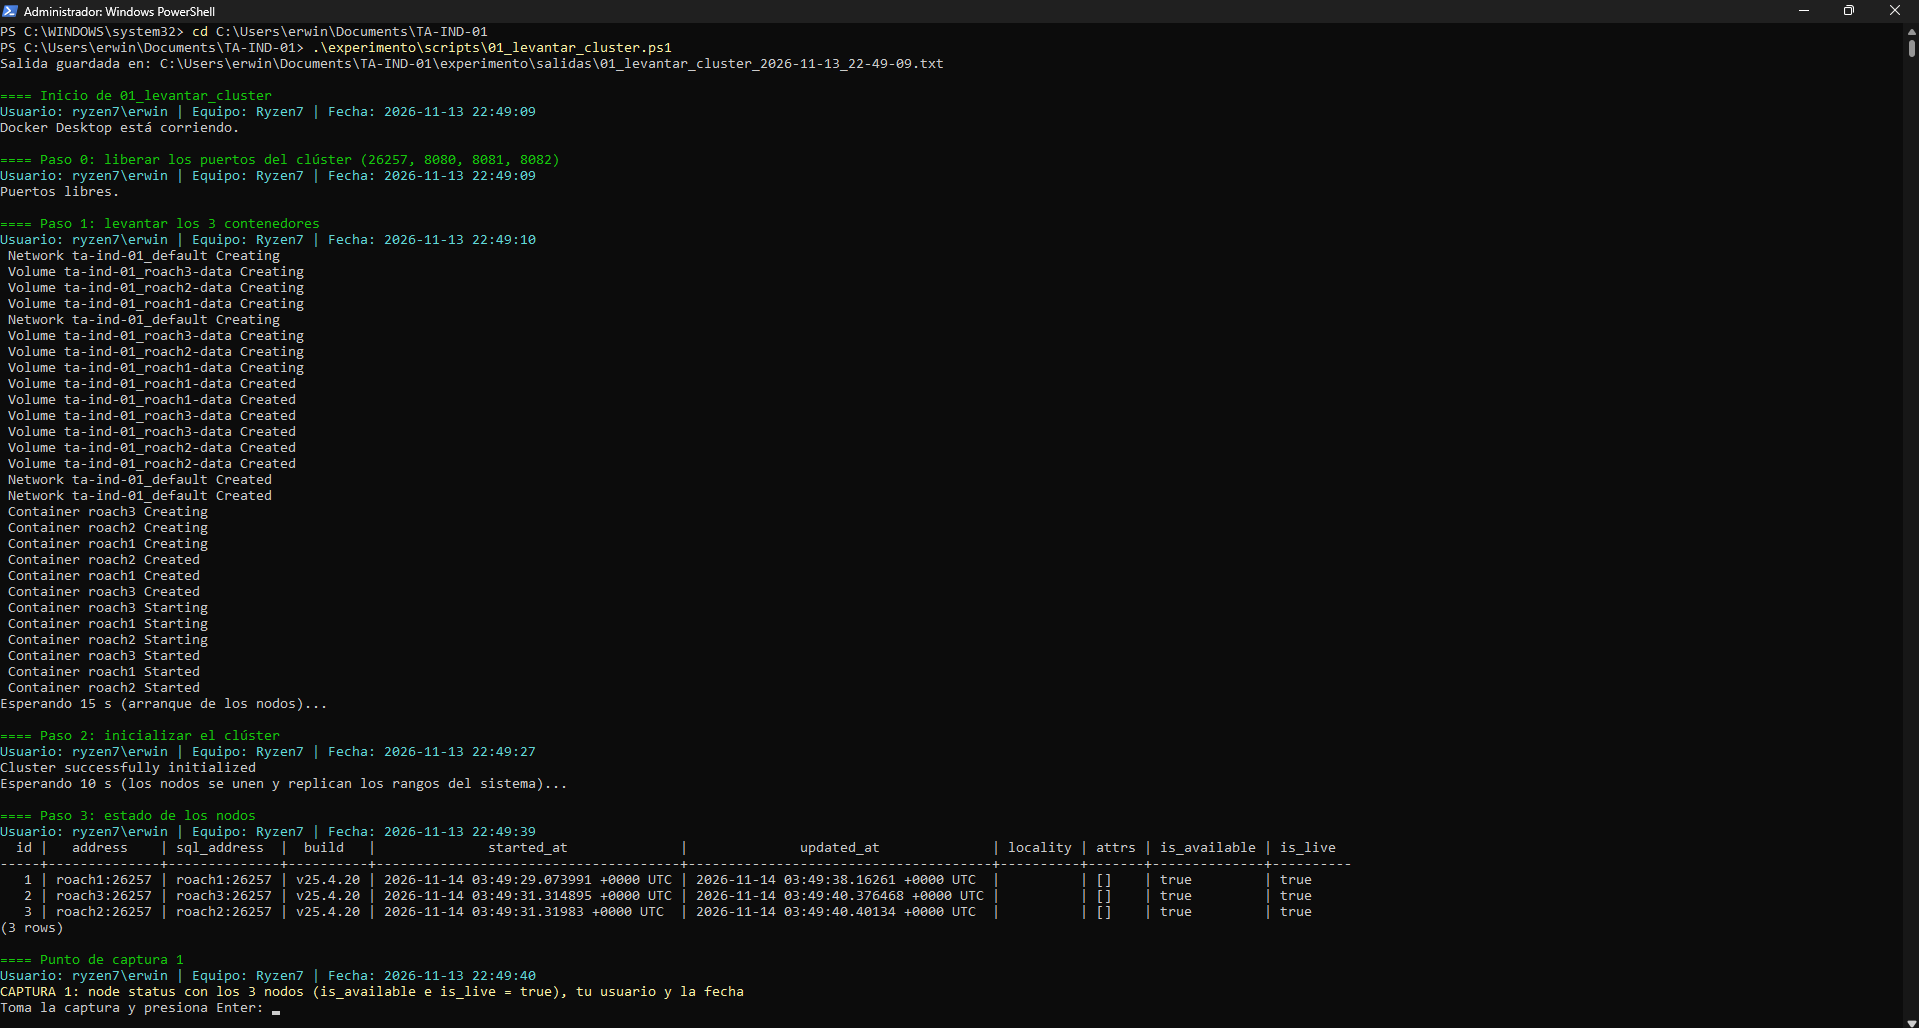
\includegraphics[width=\textwidth]{cap1_nodos.png}
  \caption{Estado inicial: tres nodos con \texttt{is\_live = true}.}
  \label{fig:nodos}
\end{figure}

\begin{figure}[H]
  \centering
  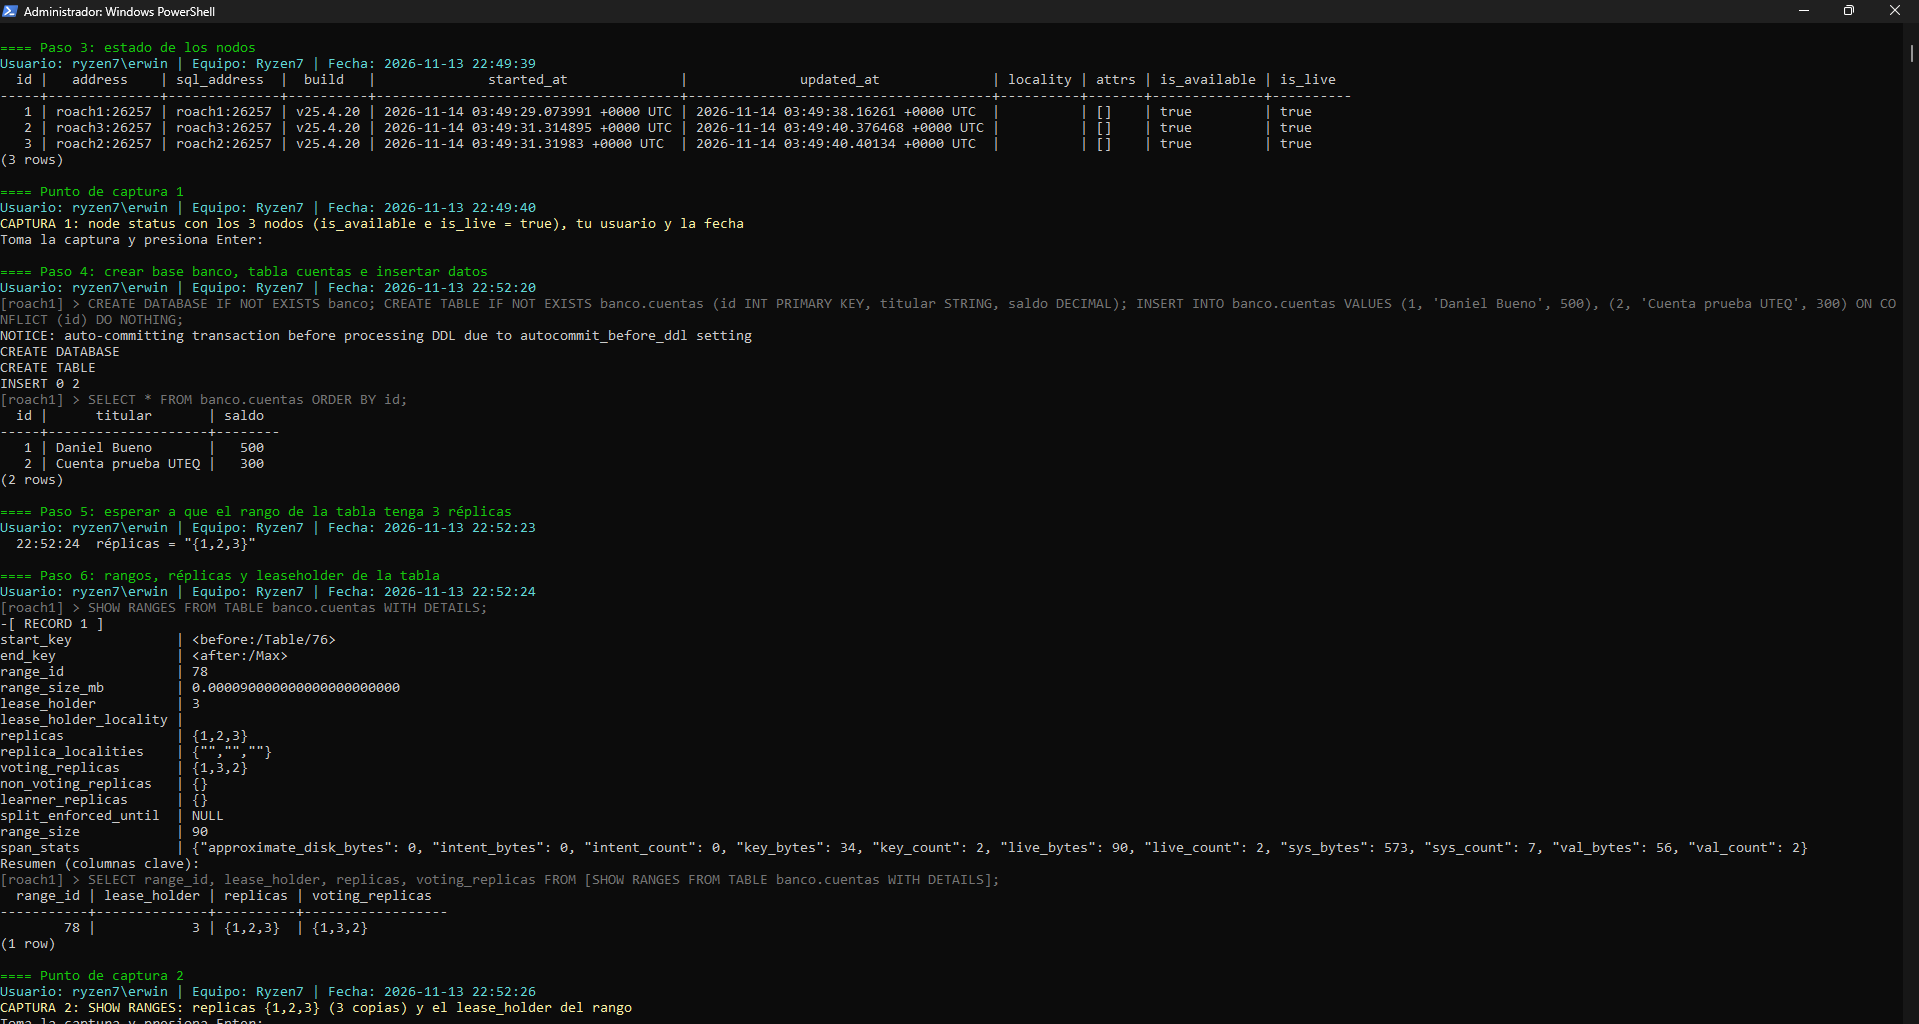
\includegraphics[width=\textwidth]{cap2_rangos.png}
  \caption{Rango r78 de \texttt{banco.cuentas} con réplicas en los tres nodos y leaseholder en el nodo 3.}
  \label{fig:rangos}
\end{figure}

\subsection{Experimento A: caída de nodos y quórum}

\begin{lstlisting}[language=bash]
docker stop roach3
cockroach sql --host=roach1 -e "INSERT INTO banco.cuentas VALUES (3,'Con un nodo caido',100)"
docker stop roach2
cockroach sql --host=roach1 -e "SET statement_timeout='10s'; SELECT * FROM banco.cuentas"
docker start roach2 roach3
\end{lstlisting}

Con roach3 apagado, \texttt{node status} lo marcó como no vivo, pero el \texttt{INSERT} de la fila 3 y el \texttt{SELECT} funcionaron (Figura~\ref{fig:quorum}). Al apagar también roach2, la consulta no respondió y terminó con el error \texttt{query execution canceled due to statement timeout} a los 11,2 segundos. El mensaje no dice \enquote{sin quórum}; esa es mi interpretación, y la sostengo porque lo único que cambió entre las dos pruebas fue pasar de dos réplicas vivas a una sola. Al encender de nuevo los nodos, la fila 3 apareció al consultar desde roach1, roach2 y roach3, así que los nodos que estuvieron apagados se pusieron al día solos.

\begin{figure}[H]
  \centering
  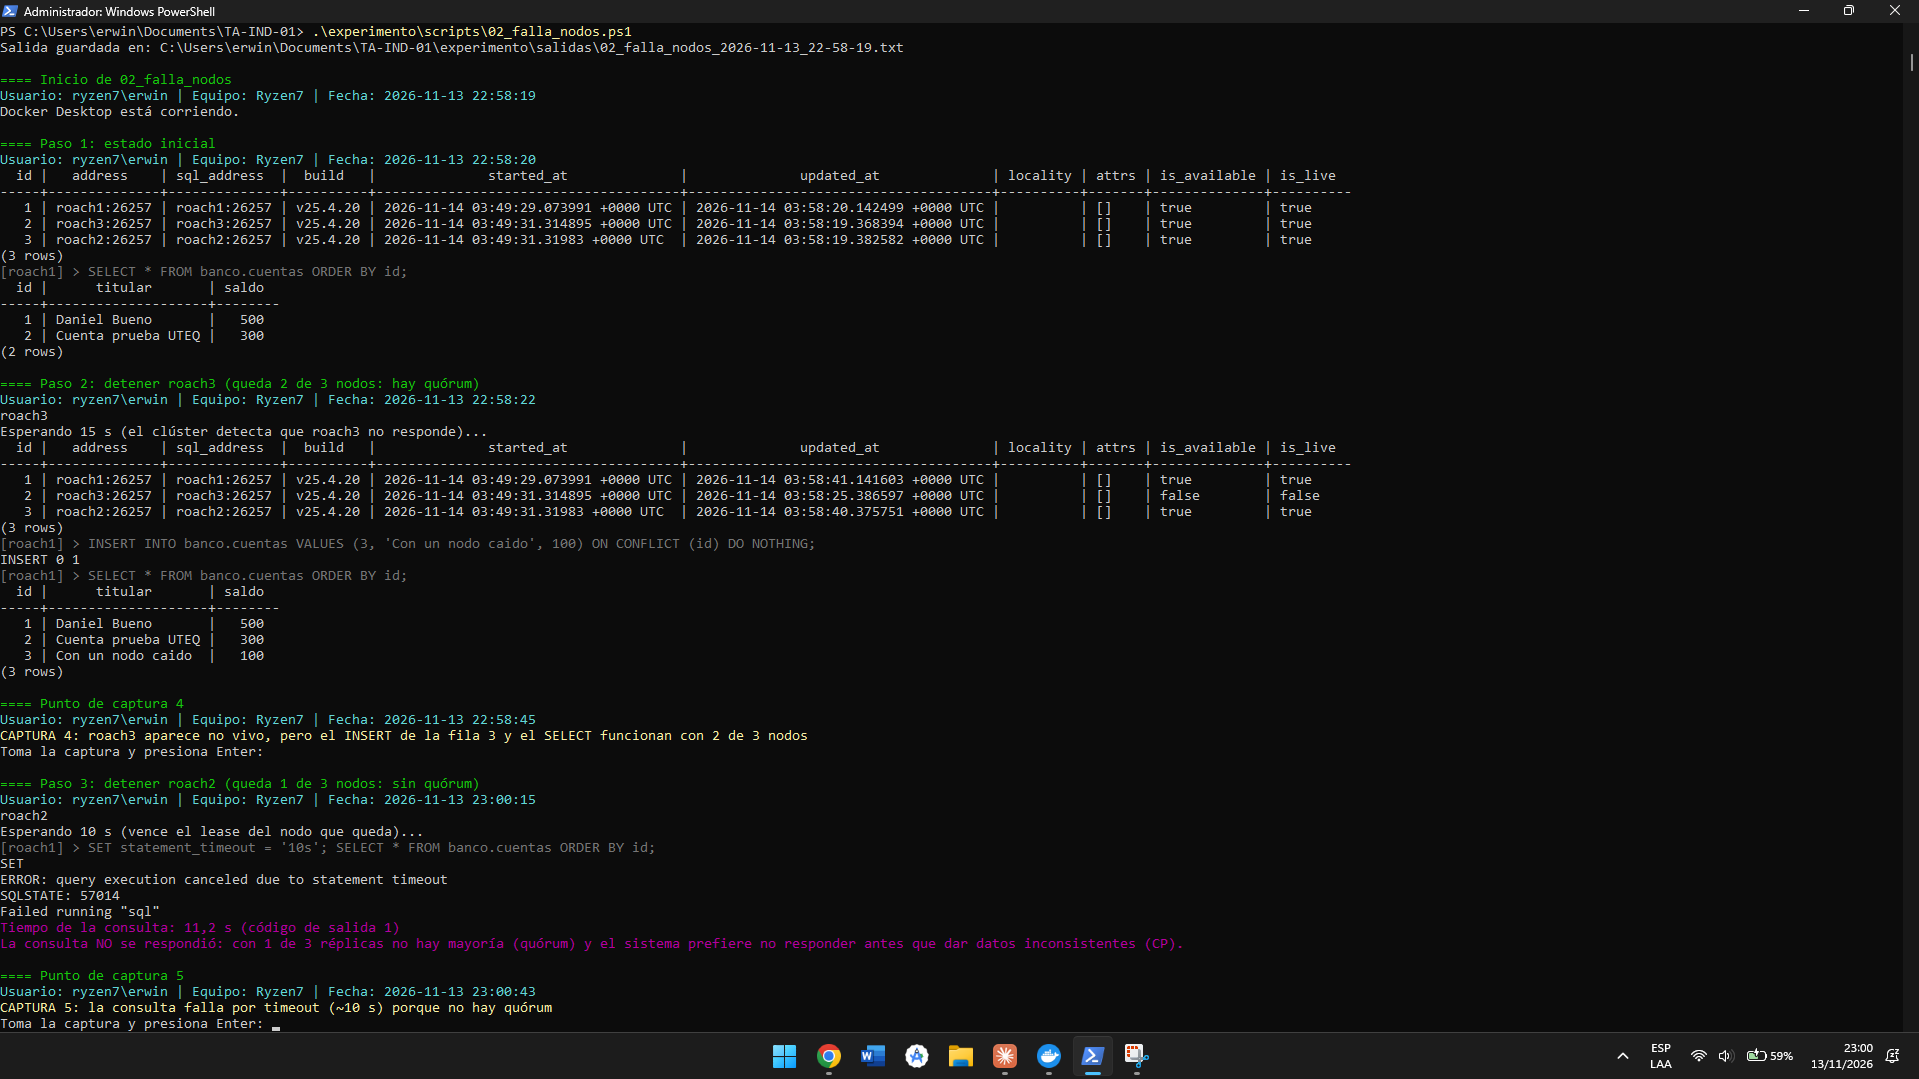
\includegraphics[width=\textwidth]{cap5_sin_quorum.png}
  \caption{Con un nodo caído el \texttt{INSERT} funciona; con dos caídos la consulta se cancela por tiempo.}
  \label{fig:quorum}
\end{figure}

Esto es la parte PC de PACELC en un caso concreto. Apagar dos contenedores no es lo mismo que una partición de red, pero para roach1 el efecto es igual: no puede hablar con la mayoría, y el sistema elige no responder.

\subsection{Experimento B: latencia frente a consistencia}

Una sesión abría una transacción que restaba 100 al saldo de la cuenta 1 y la dejaba abierta 8 segundos. Mientras tanto, otra sesión hacía dos lecturas de la misma fila: una normal y otra con \texttt{AS OF SYSTEM TIME '-5s'}. Repetí la prueba cinco veces.

\begin{table}[H]
  \centering
  \caption{Tiempo de respuesta de las lecturas con la transacción abierta (5 intentos).}
  \label{tab:latencias}
  \begin{tabular}{lrrrl}
    \toprule
    Tipo de lectura & Promedio (ms) & Mín. (ms) & Máx. (ms) & Saldo leído \\
    \midrule
    Histórica (\texttt{-5s}) & 900 & 839 & 970 & valor anterior \\
    Consistente & 6272 & 6196 & 6332 & valor nuevo \\
    \bottomrule
  \end{tabular}
\end{table}

\begin{figure}[H]
  \centering
  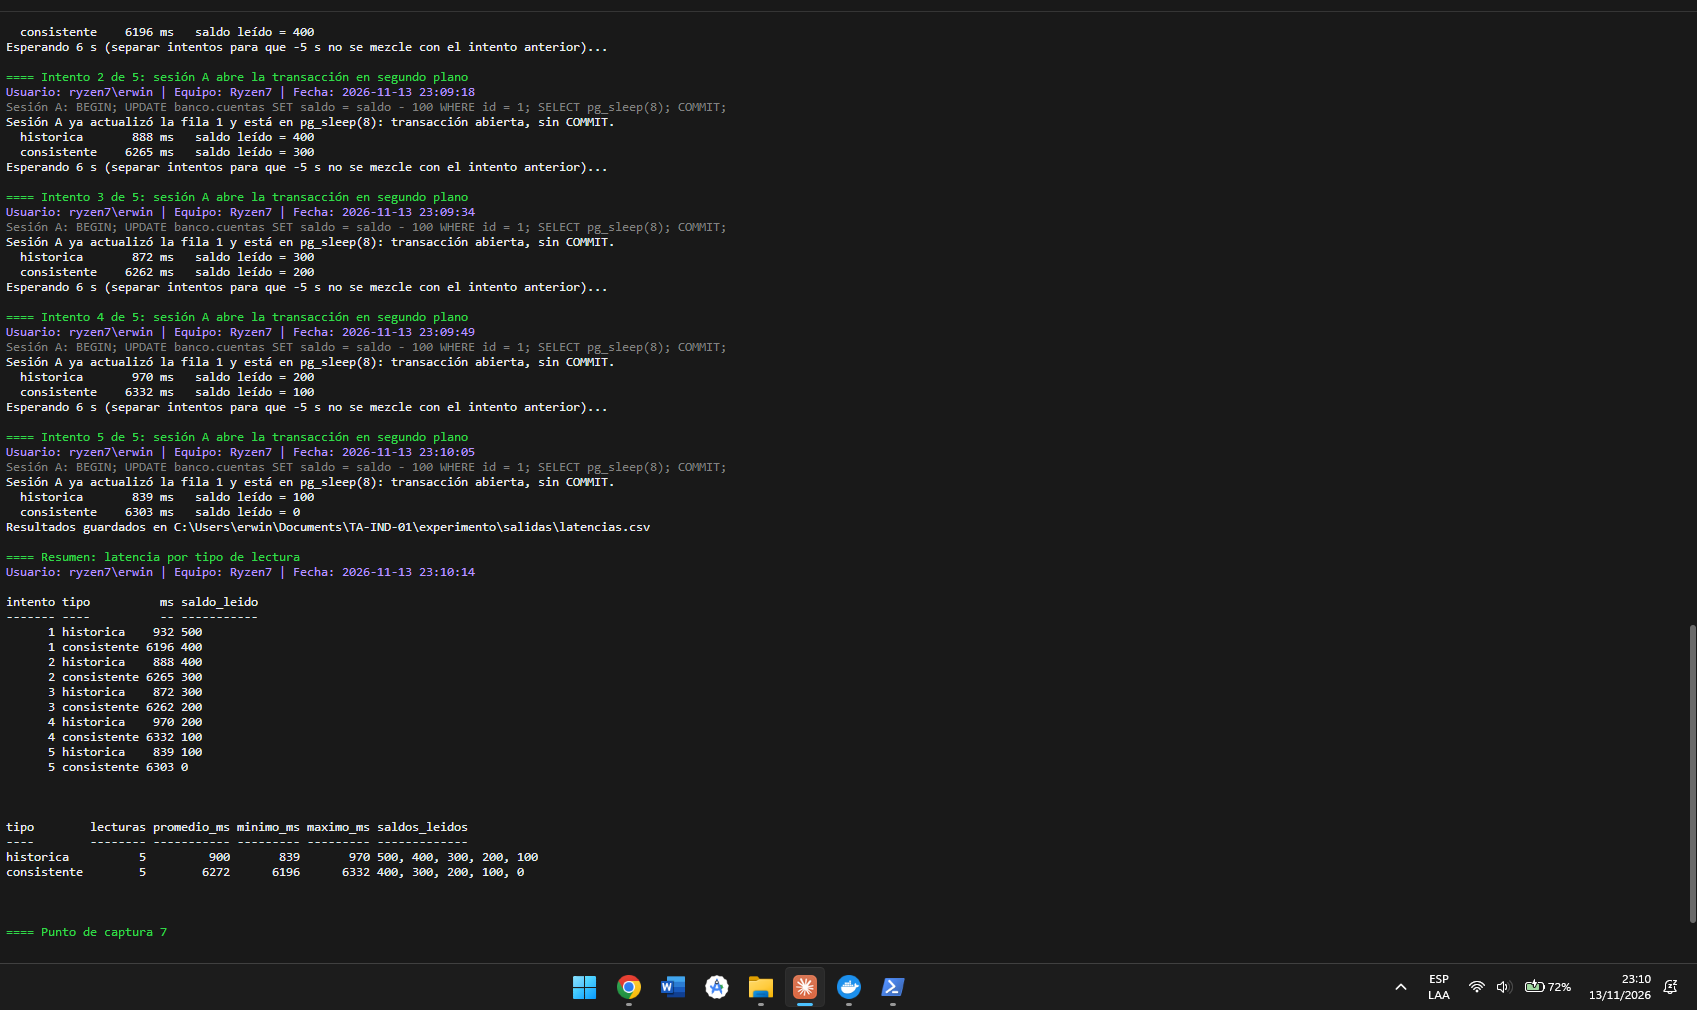
\includegraphics[width=0.95\textwidth]{cap7_latencias.png}
  \caption{Resultados del experimento B.}
  \label{fig:latencias}
\end{figure}

La lectura consistente esperó a que la transacción terminara y devolvió el saldo nuevo; la histórica respondió de inmediato con el saldo anterior (Tabla~\ref{tab:latencias}). Hay que aclarar que los 900 ms de la lectura histórica no son el tiempo de la consulta: casi todo es lo que tarda \texttt{docker exec} en arrancar el cliente, y ese costo es igual en los dos casos. Lo que importa es la diferencia, de unos 5,4 segundos, que es el tiempo que la lectura consistente pasó esperando a que la otra transacción confirmara. Es la parte EC de PACELC: aun sin fallos, quien quiere el dato más reciente paga en latencia.

% ---------------------------------------------------------------
\section{Ejemplos del entorno del estudiante}

\subsection{SGA de la UTEQ}

Me ha pasado que entro al SGA a ver mis notas y la página no carga. En las semanas de matrícula es peor: el sistema se pone muy lento o directamente se cae. No sé cómo está armado por dentro, pero lo que se ve desde afuera se repite cada vez. Todos entramos al mismo tiempo, las páginas no cargan y la gente recarga una y otra vez, así que la carga sube justo cuando el sistema está más débil. Lo relaciono con la escalabilidad y con la tolerancia a fallos de la Unidad 1. Si todo depende de un solo servidor de base de datos, la carga de la matrícula no se puede repartir, y cuando ese servidor se satura se cae el servicio entero. En CockroachDB la carga se repartiría entre varios leaseholders, aunque una tabla que todos consultan seguiría cargando más a los nodos que tienen sus rangos.

\subsection{Banca móvil de Banco Pichincha}

En la aplicación de Banco Pichincha me ha tocado que algunos módulos no funcionen. Por ejemplo, la administración de tarjetas da error, pero las transferencias siguen andando. No soy el único: el 4 de agosto de 2025 la aplicación volvió a fallar, algunos usuarios veían el mensaje \enquote{Ingreso no disponible} y otros sí podían entrar, pero no veían su saldo ni podían transferir, pagar servicios ni pagar tarjetas \cite{vistazo2025pichincha}. Según la misma nota, ya había pasado algo parecido el 25 de julio, y la Superintendencia de Bancos abrió una supervisión técnica \cite{vistazo2025pichincha}.

Tanto lo que yo vi como lo que cuenta la nota es un fallo parcial: unos servicios se caen y otros siguen funcionando. Supongo que cada módulo depende de un servicio distinto y por eso el fallo de uno no arrastra a los demás. Si lo miro con las transparencias de la Unidad 1, el fallo está a la vista (el usuario ve el error), pero queda contenido. Además veo algo parecido a lo de CockroachDB con dos nodos caídos: cuando un módulo no puede garantizar la operación, la app prefiere no mostrar el saldo o no dejar transferir antes que mostrar un dato equivocado. Lo que no veo es una recuperación automática como la de mi clúster, porque la falla volvió a aparecer en días distintos.

% ---------------------------------------------------------------
\section{Análisis comparativo}

\begin{table}[H]
  \centering
  \small
  \caption{Comparación entre CockroachDB y Google Spanner con criterios de la Unidad 1.}
  \label{tab:comparacion}
  \begin{tabular}{>{\raggedright\arraybackslash}p{3.3cm}>{\raggedright\arraybackslash}p{5.6cm}>{\raggedright\arraybackslash}p{5.6cm}}
    \toprule
    \textbf{Criterio} & \textbf{CockroachDB} & \textbf{Google Spanner} \\
    \midrule
    Replicación y consenso & Raft por rango; la escritura necesita un quórum de réplicas \cite{pina2023newsql, ajmani2022demo} & Almacén multiversión; transacciones con bloqueo y \emph{commit} en dos fases \cite{song2025k2} \\
    \addlinespace
    Orden del tiempo & Depende de que el desfase de relojes esté acotado \cite{ajmani2022demo} & TrueTime con incertidumbre acotada (unos 7 ms) \cite{song2025k2} \\
    \addlinespace
    CAP / PACELC & PC/EC; lecturas históricas opcionales con \texttt{AS OF SYSTEM TIME} \cite{ajmani2022demo} & PC/EC; serializabilidad estricta y lecturas de instantánea sin bloqueo \cite{song2025k2} \\
    \addlinespace
    Transparencia de ubicación & Total en una región; en multirregión se declara la localidad con SQL \cite{vanbenschoten2022multiregion} & Almacén de escala global; el cliente usa la API sin elegir réplica \cite{song2025k2} \\
    \addlinespace
    Tolerancia a fallos & Sobrevive a una zona por defecto y a una región si se configura \cite{ajmani2022demo} & Las fuentes usadas no detallan su configuración de réplicas \\
    \addlinespace
    Modelo de comunicación & Cliente-servidor con protocolo PostgreSQL; nodos iguales con RPC y gossip & Cliente-servidor; varias rondas síncronas por transacción de escritura \cite{song2025k2} \\
    \addlinespace
    Despliegue & Local, en cualquier nube o como servicio gestionado \cite{swenson2025serverless} & Servicio de Google Cloud \\
    \bottomrule
  \end{tabular}
\end{table}

Los dos sistemas toman las mismas decisiones de fondo: consenso por mayoría, consistencia antes que disponibilidad y lecturas de una versión anterior como válvula de escape para la latencia. Donde se separan es en el reloj. Spanner puede confiar en TrueTime porque Google controla el hardware de sus centros de datos. CockroachDB tiene que correr en un servidor cualquiera, por eso necesita que el desfase entre relojes esté acotado y lo trata como una condición de su consistencia \cite{ajmani2022demo}. La otra diferencia importante es el despliegue: Spanner amarra la aplicación a Google Cloud, mientras que con CockroachDB pude reproducir el comportamiento del sistema en mi laptop.

CockroachDB también tiene una salida para leer cerca del usuario sin encarecer las escrituras. Las réplicas seguidoras reducen la latencia de lectura, pero si todas votan, el leaseholder tiene que replicar en un quórum más grande. Por eso distingue entre seguidores con voto y sin voto, y así aumenta el número de copias sin aumentar el quórum \cite{ajmani2022demo}.

% ---------------------------------------------------------------
\section{Postura crítica}

Lo mejor de CockroachDB, para mí, es que da transacciones serializables sobre datos distribuidos sin pedir hardware especial. Lo comprobé: perdí un nodo y no perdí ni una escritura, y cuando los nodos volvieron los tres tenían los mismos datos. En un sistema de pagos o de inventario, donde un saldo duplicado cuesta dinero, prefiero esa garantía aunque cueste unos milisegundos.

El primer problema es la latencia. Cada escritura necesita una ronda de consenso, y en mi experimento B una lectura normal se quedó más de 5 segundos esperando detrás de una transacción abierta. En la evaluación de Pina et al., que comparó CockroachDB con MariaDB Xpand y VoltDB, CockroachDB fue el que mejor escaló y el que cargó los datos más rápido, pero VoltDB ejecutó las consultas en menos tiempo \cite{pina2023newsql}. O sea, CockroachDB se elige por la escala y las garantías; si lo que importa es la velocidad de cada consulta, hay opciones mejores.

También está la disponibilidad. Con dos de tres nodos caídos el sistema deja de responder, y lo hace a propósito. Hay aplicaciones donde un dato un poco viejo no le hace daño a nadie, como un contador de vistas o el catálogo de una tienda. Ahí esa rigidez es un costo que no hace falta pagar, y una base AP como Cassandra encaja mejor \cite{ahmed2023consistency}.

Me preocupa además la dependencia del reloj. Las garantías de CockroachDB suponen que el desfase entre relojes está acotado \cite{ajmani2022demo}, y en servidores comunes eso queda en manos de la sincronización por red. Spanner tiene ese punto mejor resuelto con TrueTime \cite{song2025k2}, pero a cambio la aplicación queda atada a Google.

Hay un límite que comparten los dos sistemas. La replicación síncrona protege contra máquinas y redes que se caen, pero no contra datos malos: si la aplicación escribe un valor equivocado, el consenso lo copia igual de bien a todas las réplicas. Para eso siguen haciendo falta validaciones y respaldos.

No usaría CockroachDB para una aplicación pequeña de un solo servidor, donde PostgreSQL es más simple y más rápido, ni para cargas analíticas pesadas, ni cuando la disponibilidad importa más que la exactitud. Sí lo usaría para datos transaccionales que no se pueden perder y que tienen que aguantar la caída de un nodo, una zona o una región entera.

% ---------------------------------------------------------------
\section{Conclusiones}

En mi clúster de tres nodos, CockroachDB siguió aceptando escrituras con un nodo caído y dejó de responder con dos. Lo que decide si el sistema aguanta es el quórum de Raft (2 de 3); la cantidad de nodos encendidos por sí sola no dice mucho.

La consistencia cuesta tiempo aun cuando no falla nada. En mi prueba, la lectura consistente tardó unos 5,4 segundos más que la histórica porque tuvo que esperar a una transacción abierta. Por eso clasifico a CockroachDB como PC/EC, y veo \texttt{AS OF SYSTEM TIME} como la forma que tiene el desarrollador de elegir latencia cuando un dato algo viejo le sirve.

Spanner y CockroachDB toman las mismas decisiones frente a CAP y PACELC. Donde de verdad se diferencian es en el reloj (TrueTime frente a relojes comunes con desfase acotado) y en dónde se pueden instalar (solo Google Cloud frente a cualquier infraestructura).

La transparencia de fallos de CockroachDB depende de que haya mayoría: con ella el fallo no se nota, sin ella el cliente recibe un error. Algo parecido vi como usuario. En la banca móvil falla un módulo y los demás siguen; en el SGA, en cambio, la sobrecarga de la matrícula tumba el servicio completo.

Mi experimento tiene un límite que hay que decir: apagué contenedores en una sola máquina, que no es lo mismo que una partición real entre centros de datos. Para medir de verdad el costo de la latencia, el siguiente paso sería repetir las pruebas con nodos en regiones distintas.

% ---------------------------------------------------------------
\section{Declaración de uso de inteligencia artificial}

Usé Claude (Anthropic), modelo Claude Opus 5.5, en la aplicación de Claude y en Claude Code, con estos fines:

\begin{itemize}
  \item Generar el archivo \texttt{docker-compose.yml} y los scripts de PowerShell del experimento.
  \item Buscar los artículos y verificar sus datos (autores, año, revista, volumen, número, páginas y DOI) contra Crossref.
  \item Pasar mi bosquejo a mano al diagrama en TikZ.
  \item Redactar un borrador del informe a partir de mis capturas, mis resultados y mis ejemplos.
\end{itemize}

Para verificar lo obtenido ejecuté yo mismo los scripts y revisé que las salidas guardadas coincidieran con lo que vi en la terminal, abrí cada DOI para confirmar que lleva a la obra citada, leí en los artículos los fragmentos que cito (Anexo~\ref{anx:lecturas}) y revisé y corregí el texto del borrador.

% ---------------------------------------------------------------
\printbibliography[title={Referencias}]

% ---------------------------------------------------------------
\appendix
\section{Esquema inicial a mano}
\label{anx:bosquejo}

\begin{figure}[H]
  \centering
  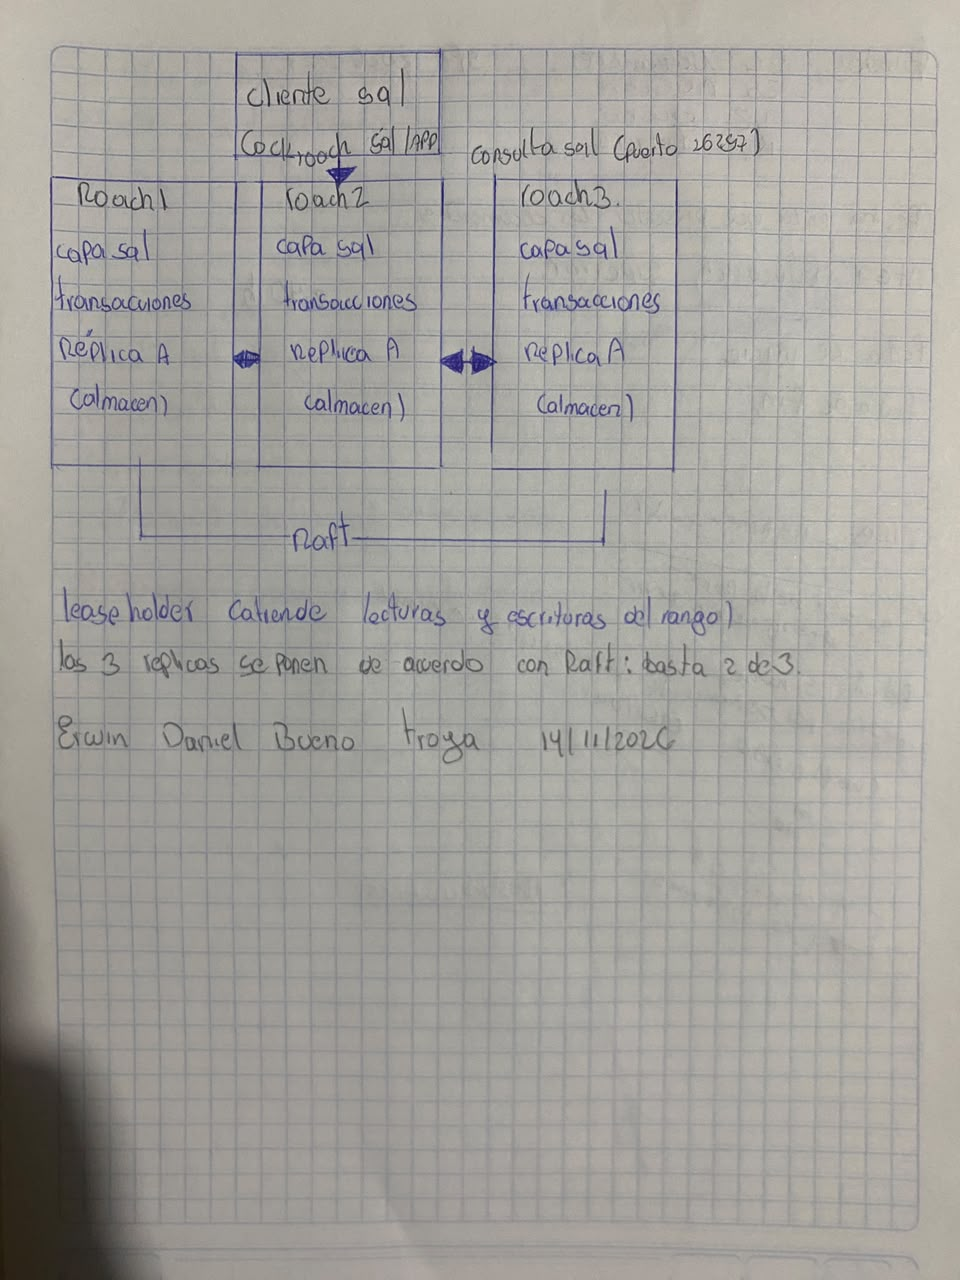
\includegraphics[width=0.7\textwidth]{bosquejo.png}
  \caption{Primer bosquejo de la arquitectura, hecho a mano el 14/11/2026.}
\end{figure}

\section{Capturas de lectura de las fuentes}
\label{anx:lecturas}

Cada captura corresponde a un fragmento citado en el informe. Las marcas a mano las hice yo al leer cada artículo.

\begin{figure}[H]
  \centering
  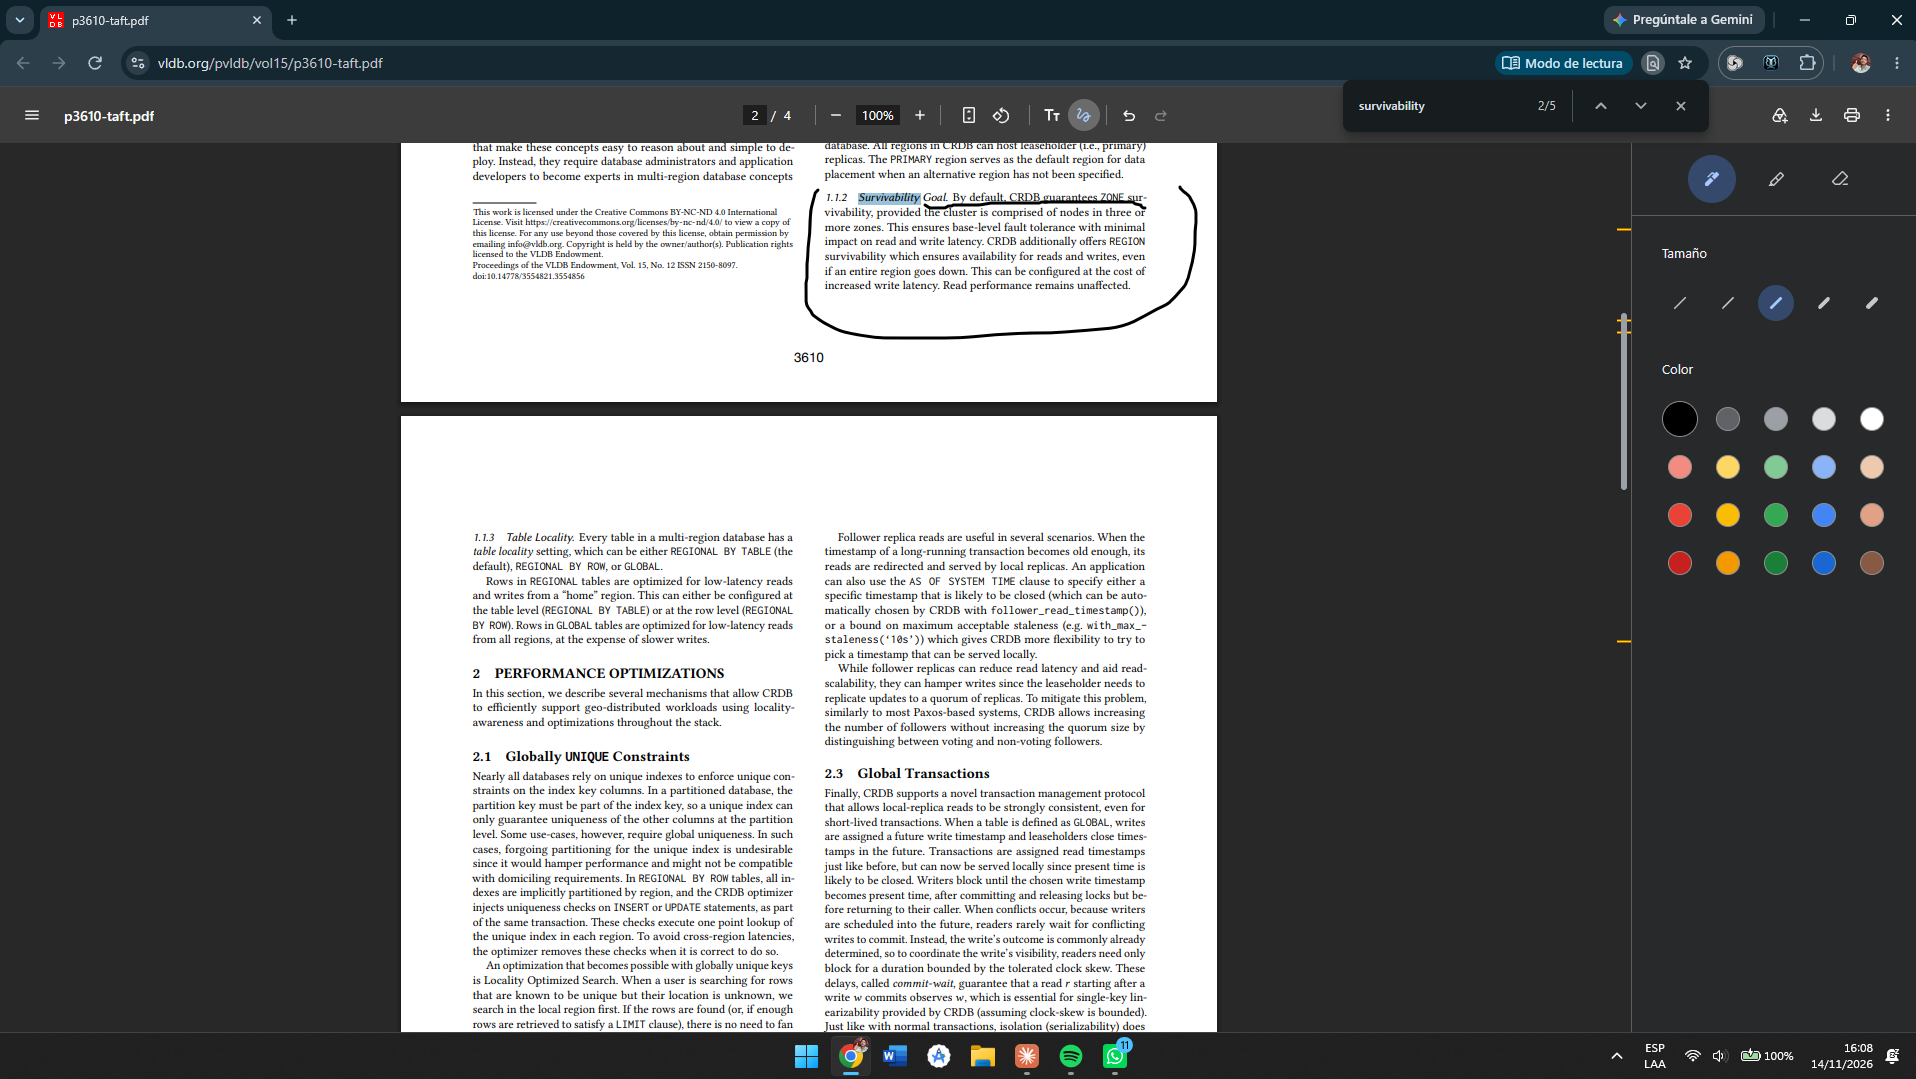
\includegraphics[width=\textwidth]{lectura1.png}
  \caption{Ajmani et al. \cite{ajmani2022demo}, p. 3610, apartado 1.1.2: supervivencia a la caída de una región a costa de mayor latencia de escritura. Citado en la sección de CAP y PACELC.}
\end{figure}

\begin{figure}[H]
  \centering
  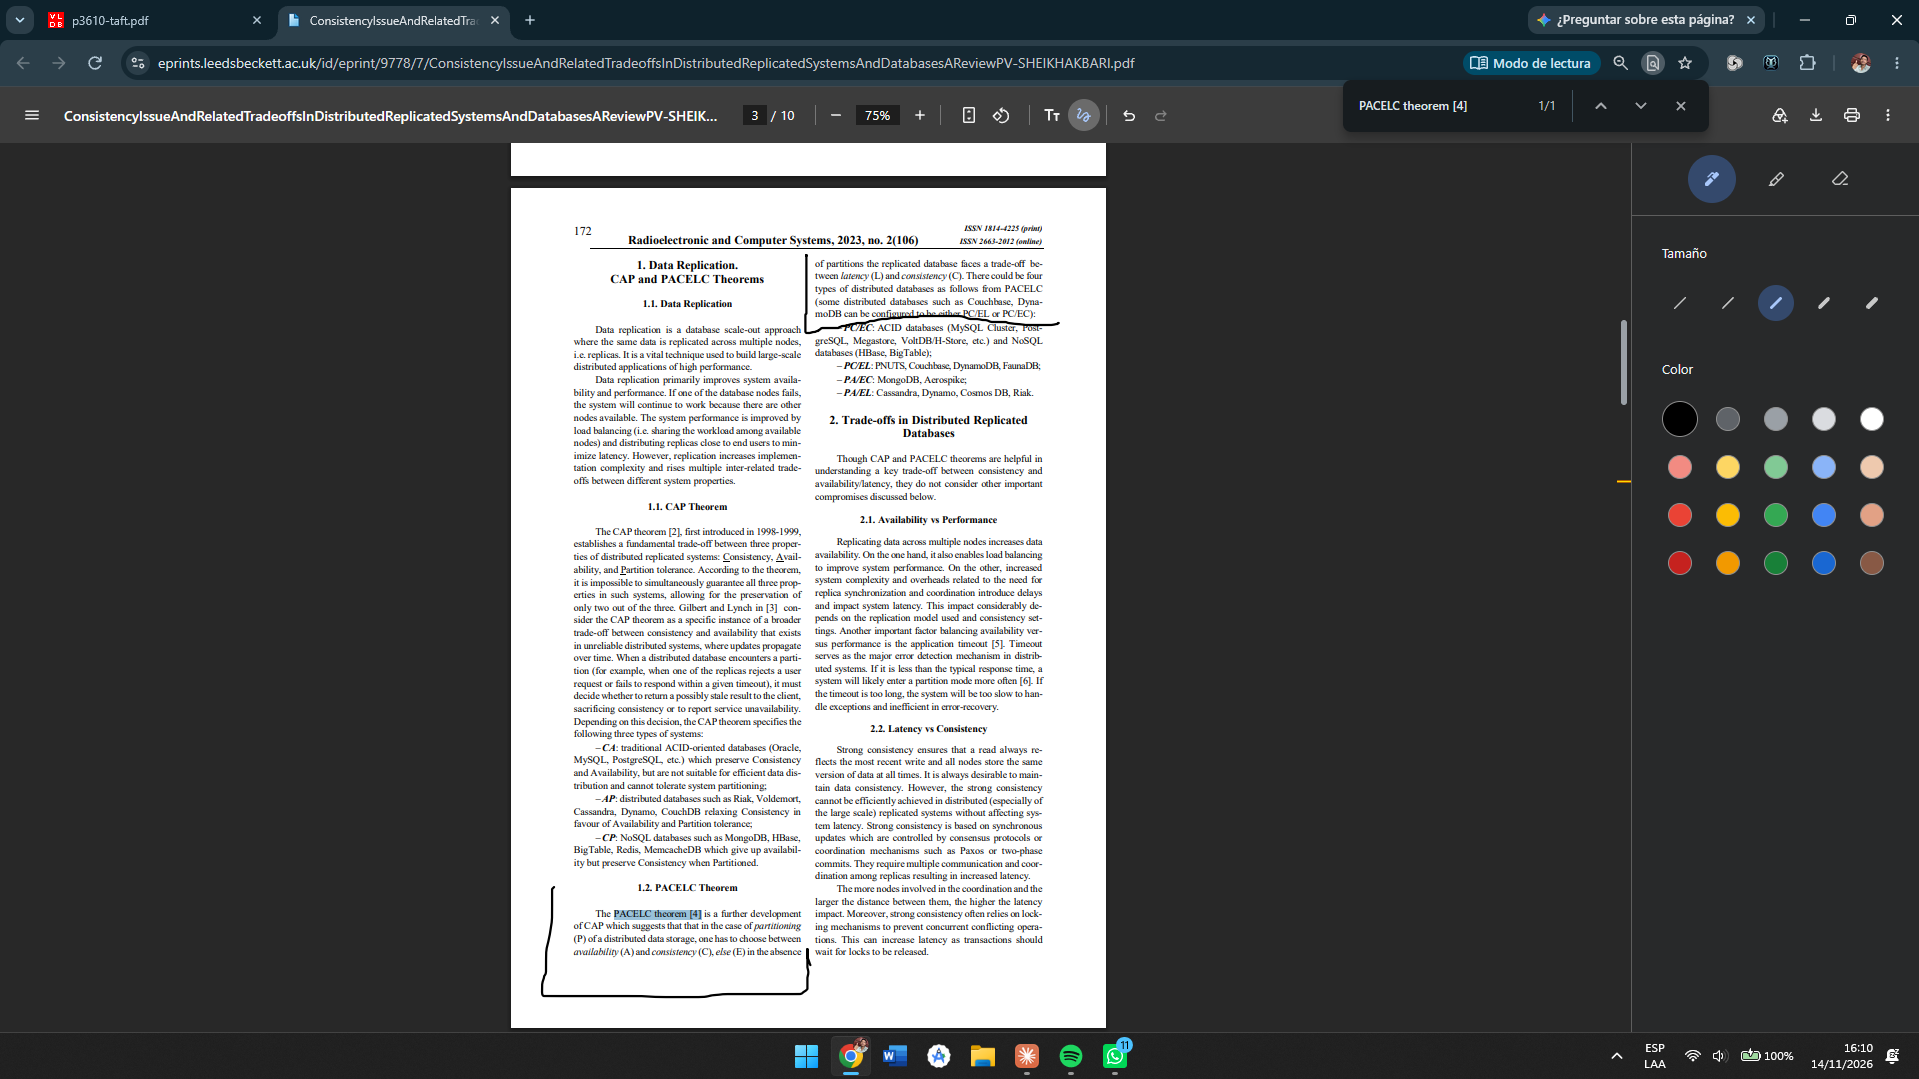
\includegraphics[width=\textwidth]{lectura2.png}
  \caption{Ahmed et al. \cite{ahmed2023consistency}, p. 172, apartado 1.2: definición de PACELC (sin partición, compromiso entre latencia y consistencia). Citado en la sección de CAP y PACELC.}
\end{figure}

\begin{figure}[H]
  \centering
  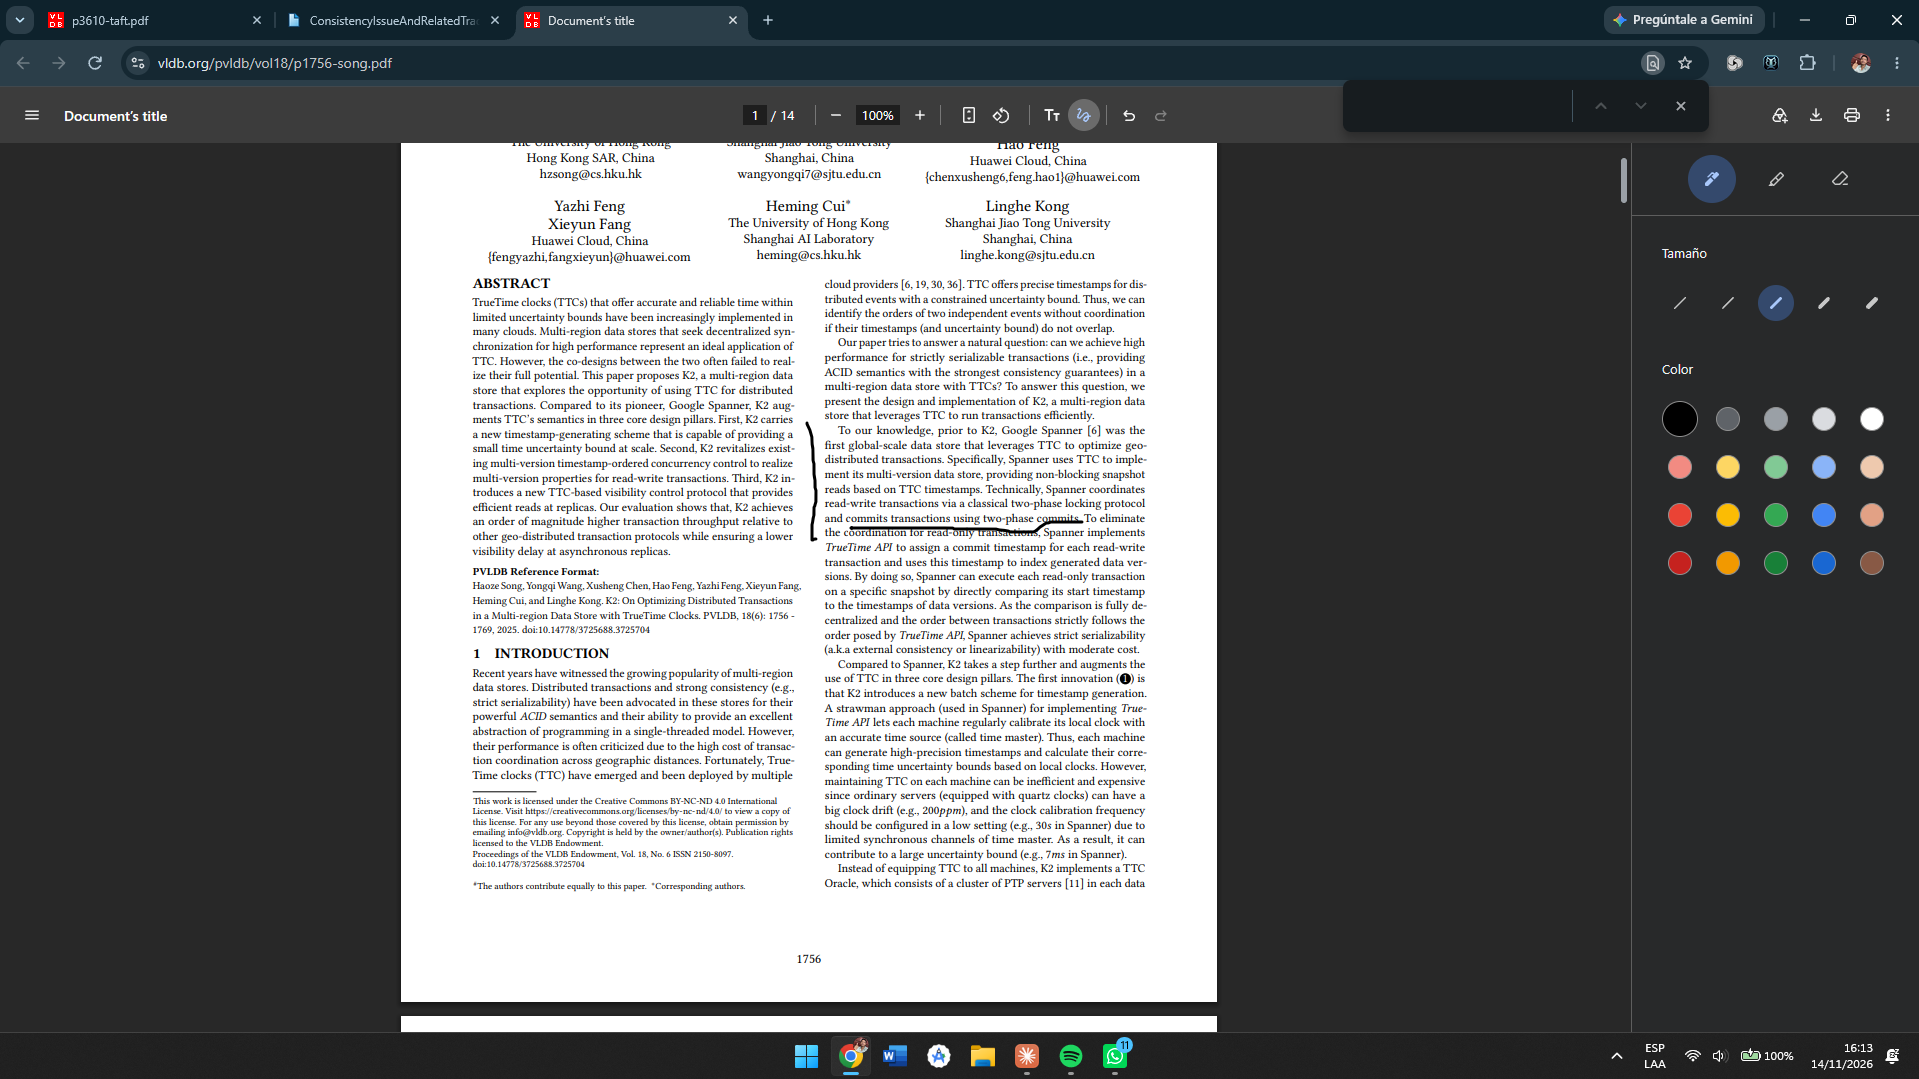
\includegraphics[width=\textwidth]{lectura3.png}
  \caption{Song et al. \cite{song2025k2}, p. 1756, introducción: Spanner usa TrueTime para lecturas no bloqueantes y coordina sus transacciones con bloqueo y \emph{commit} en dos fases. Citado en las secciones de CAP y PACELC y de modelos de comunicación.}
\end{figure}

\end{document}
